\chapter{Logic in Computer Science}

\section{First-Order Logic}

\begin{defi}[Signature]
$S$ is a \term{signature} if $S$ is a four-tuple \tuple{P,F,r,C} where:
\begin{enumerate}
\item $P$ is a set of \term{predicate symbols} \brak{P_1,P_2,\ldots,P_n},
\item $F$ is a set of \term{function symbols} \brak{F_1,F_2,\ldots,F_m},
\item $r$ is \term{arity} or \term{degree of functions} and relations. For each $P_i$ respectively $F_j$, \fun{r}{P_i} respectively \fun{r}{F_j} is a non-zero natural number denoting the arity of $P_i$ respectively $F_j$,
\item $C$ is a set of \term{constant symbols}.
\end{enumerate}
\cite{conf/fedcsis/Telnarova12}
\end{defi}

\begin{defi}[Alphabet]
An \term{alphabet} $\Sigma$ consists of the following symbols:
\begin{enumerate}
\item Signature $S=\tuple{P,F,r,C}$.
\item \term{Collection of variables} $V$.
\item \term{Operators}: $\neg$ (\term{negation}), $\wedge$ (\term{conjunction}), $\vee$ (\term{disjunction}), $\rightarrow$ (\term{implication}), $\leftrightarrow$ (\term{equivalence}).
\item \term{Quantifiers}: $\forall$ (\term{forall}), $\exists$ (\term{exists}).
\item \term{Parentheses} and \term{punctuation symbols}: $($, $)$ and $,$.
\end{enumerate}
\cite{conf/fedcsis/Telnarova12}
\end{defi}

\begin{defi}[Term]
A \term{term} is defined inductively as follows:
\begin{enumerate}
\item Variable is term.
\item Constant is term.
\item If $f$ is a function symbol ($f\in F$) with arity $m$ and $t_1,t_2,\ldots,t_m$ are terms of $\Sigma$, then \ffun{t_1,t_2,\ldots,t_m} is term of $\Sigma$.
\end{enumerate}
\cite{conf/fedcsis/Telnarova12}
\end{defi}

\begin{defi}[Atom]
If $p$ is predicate symbol with arity $m$ and $t_1,t_2,\ldots,t_m$ are terms of $\Sigma$, then $\fun{p}{t_1,t_2,\ldots,t_m}$ is an \termor{atomic formula}{atom}. An atomic formula is a \term{formula} and all occurrences of variables in an atomic formula are free.
\cite{conf/fedcsis/Telnarova12}
\end{defi}

\begin{defi}[Formula]
A \term{formula} is defined as follows:
\begin{enumerate}
 \item An atom is a formula.
 \item If $H$ and $G$ are formulas, then:
 \begin{enumerate}
  \item $\neg H$ is a formula, the occurrence of variables in $\neg H$ is free respectively bound if it is free respectively bound in $H$,
  \item $H\wedge G$ is a formula, the occurrence of variables in $H\wedge G$ is free respectively bound if it is free respectively bound in $H$ or $G$,
  \item $H\vee G$ is a formula, the occurrence of variables in $H\vee G$ is free respectively bound if it is free respectively bound in $H$ or $G$,
  \item $H\rightarrow G$ is a formula, the occurrence of variables in $H\rightarrow G$ is free respectively bound if it is free respectively bound in $H$ or $G$,
  \item $H\leftrightarrow G$ is a formula, the occurrence of variables in $H\leftrightarrow G$ is free respectively bound if it is free respectively bound in $H$ or $G$.
 \end{enumerate}
 \item If $H$ is a formula and $x$ is a variable, then $\forall x:H$ and $\exists x:H$ are formulas. All occurrences of $x$ are bound.
\end{enumerate}
\cite{conf/fedcsis/Telnarova12}
\end{defi}

\begin{defi}[Literal]
A \term{literal} $L$ is an atom or the negation of an atom.
\cite{conf/fedcsis/Telnarova12}
\end{defi}

\begin{defi}[Clause]
A \term{clause} is a formula such as $\forall\vec{x}:L_1\vee L_2\vee\ldots\vee L_m$ where each $L_i$ is a literal and $\vec{x}=\brak{x_1,x_2,\ldots,x_n}$ are all the variables occurring in $L_1\vee L_2\vee\ldots\vee L_m$.
\cite{conf/fedcsis/Telnarova12}
\end{defi}

\begin{defi}[Horn-clauses]
\term{Horn-clause}s have the form: $\forall x_1,x_2,\ldots,x_n:L_1\wedge L_2\wedge\ldots\wedge L_m\rightarrow L$ where $L,L_1\wedge L_2\wedge\ldots\wedge L_m$ are a literals and $x_1,x_2,\ldots,x_n$ are all variables having free occurrences in $L,L_1\wedge L_2\wedge\ldots\wedge L_m$.
\cite{conf/fedcsis/Telnarova12}
\end{defi}

\begin{defi}[Negation of a dilemma, Conjunction of dilemmas, Disjunction of dilemmas]
For a given set $D$ of dilemmas it is defined:
\begin{enumerate}
 \item A \term{negation of a dilemma} $d=\dilemma{u}$ as a dilemma $\neg d=\negdilemma{u}$;
 \item A \term{disjunction of the dilemmas} $d'=\dilemma{u'}$, $d''=\dilemma{u''}$ as a dilemma $d'\vee d''=\flatbrak{u'\vee u''|\neg\brak{u'\vee u''}}$;%
 \item A \term{conjunction of the dilemmas} $d'=\dilemma{u'}$, $d''=\dilemma{u''}$ as a dilemma $d'\wedge d''=\flatbrak{u'\wedge u''|\neg\brak{u'\wedge u''}}$;%
\end{enumerate}
\cite{conf/fedcsis/Kulikowski12}
\end{defi}

\begin{defi}[Equal certainty relation, Ambivalent dilemma, Equivalent dilemmas, Anti-equivalent dilemmas]
Let $D$ be a set of dilemmas. Then in $D$ a binary relation $\approx^c$ satisfying the conditions of:
\begin{enumerate}
\item Reciprocity: for each $d\in D$ it holds $d\approx^c d$;
\item Symmetry: for any $d',d''\in D$ if $d'\approx^c d''$ then also $d''\approx^c d'$ holds;
\item Reflexivity: for any $d',d''\in D$ if $d'\approx^c d''$ then also $\neg d'\approx^c\neg d''$ holds;
\item Transitivity: for any $d',d'',d'''\in D$ if $d'\approx^c d''$ and $d''\approx^c d'''$ then also $d'\approx^c d'''$ holds;
\item Fixation: for any $d',d''\in D$ if $d'\approx^c\neg d'$ and $d''\approx^c\neg d''$ then also $d'\approx^c d''$ holds,
\end{enumerate}
will be called an \term{equal certainty relation}. Any dilemma satisfying the condition $d\approx^c\neg d$ will be called an \term{ambivalent dilemma}; any dilemmas such that $d'\approx^c d''$ holds will be called \term{equivalent dilemmas}; any dilemmas such that $d'\approx^c\neg d''$ holds will be called \term{anti-equivalent dilemmas}.
\cite{conf/fedcsis/Kulikowski12}
\end{defi}

\begin{defi}[Certainty ranking]
Let $D$ be a set of dilemmas with established equal certainty relation. Then a binary relation $\preceq^c$ described in $D$ and satisfying the conditions of:
\begin{enumerate}
 \item reciprocity: for each $d\in D$ it holds $d\preceq^c d$;
 \item symmetry: for any $d',d''\in D$ $d'\preceq^c d''$ and $d''\preceq^c d'$ hold if and only if $d'\approx^c d''$ holds;
 \item anti-reflexivity: for any $d',d''\in D$ if $d'\preceq^c d''$ then $\neg d''\preceq^c\neg d'$ holds;
 \item transitivity: for any $d',d'',d'''\in D$ if $d'\preceq^c d''$ and $d''\preceq^c d'''$ then also $d'\preceq^c d'''$ holds,
\end{enumerate}
will be called a \term{certainty ranking}.
\cite{conf/fedcsis/Kulikowski12}
\end{defi}

\begin{theo}
Let $D$ be a set of dilemmas with established equal certainty and certainty ranking relations. Then for any $d',d''\in D$:
\begin{enumerate}
\item if $d'\preceq^c d''$ and not $d''\preceq^c d'$ then $d'\vee d''\preceq^c d''$;
\item if $d'\preceq^c d''$ and not $d''\preceq^c d'$ then $d'\wedge d''\preceq^c d'$;
\item if $d'\approx^c d''$ then $d'\vee d''\approx^c d'\wedge d''\approx^c d'\approx^c d''$;
\item if $d'\approx^c d''$ then $d'\wedge d''\approx^c d',d''$;
\item if $d'\approx^c d''$ then $d',d''\approx^c d'\vee d''$
\end{enumerate}
\cite{conf/fedcsis/Kulikowski12}
\end{theo}

\section{Logic Programming}

\begin{defi}[Domain declaration for predicate symbol $p$]
A \term{domain declaration for predicate symbol $p$} of arity n is an expression of the following form.
\begin{equation}
\mbox{domain }\fun{p}{a_1,\ldots ,a_n}
\end{equation}
where $a_i$ is either $h$ or $d$. When $a$ is equal to $h$, this means that the $i$-th argument of $p$ ranges over the Herbrand universe. Otherwise, it means that the $i$-th argument is a list of variables which ranges over $d_1$ In the following, the domains $d_i$ are finite and explicit sets of values (i.e constants).
\cite{conf/ijcai/Hentenryck87}
\end{defi}

\begin{defi}[Domain set of a logic program]
Let $dl,\ldots ,dn$ the domains appearing in the domain declarations of a logic program $PR$ and different from the Herbrand universe. We note \fun{D}{PR} the set $\accol{d|d\neq\emptyset\wedge d\in 2^{d_i}\accol{1\leq i\leq n}}$ We call it the \term{domain set of the logic program}. The domain set of a logic program contains all domains we possibly need during the computations.
\cite{conf/ijcai/Hentenryck87}
\end{defi}

\begin{defi}[Range of a term included in a domain]
We say that the \term{range of $t$ is included in a domain $d_t$} denoted $\abs{t}\in d_i$ if $t$ is a constant $\in d_t$ or a $d$-variable $x^{d_t}$ such that $d_t\subseteq d$
\cite{conf/ijcai/Hentenryck87}
\end{defi}

\begin{defi}[$d$-substitution]
A $d$-substitution $\theta$ is a finite set of the form $\accol{v_1/t_1,\ldots,v_n/t_n}$ where
\begin{enumerate}
 \item each $v_i$ is either a variable or $d$-variable
 \item $t_i$ is a term distinct from $v_i$,
 \item $v_1,\ldots,v_n$ are all distinct,
 \item if $v_i$ is a $d$-variable $v^{d_i}$, $\abs{t_i}\in d_i$
\end{enumerate}
\cite{conf/ijcai/Hentenryck87}
\end{defi}

\begin{defi}[$d$-substitutions agree on a set of variables and $d$-variables]
We say that two \term[$d$-substitutions agree on a set of variables and $d$-variables]{$d$-substitutions $\theta$ and $\lambda$ agree on a set $V$ of variables and $d$-variables}, denoted $\theta=\lambda\abs{V}$ \iffTx{} $x\theta=x\lambda$ for each $x\in V$ where $=$ denotes syntactic equality.
\cite{conf/ijcai/Hentenryck87}
\end{defi}

\begin{defi}[$d$-instance]
$\theta$ is a \term{$d$-instance} of $\lambda$ in $V$, denoted $\lambda\leq\theta$ \iffTx{} $x\theta=\delta\circ\lambda$ for some $d$-substitution $\delta$.
\cite{conf/ijcai/Hentenryck87}
\end{defi}

\begin{defi}[$d$-unifier, unifies, more general $d$-unifier, $d$-mgu]
A $d$-substitution $\sigma$ is a \term{$d$-unifier} of some non-empty and finite subset $S=\accol{t_1,\ldots,t_n}$ where $t_i$ and a literal of a term \iffTx{} $t_1\sigma=\ldots=t_n\sigma$, we also say that $\sigma$ \term{unifies} $S$. \term{\fun{UNI}{S}} is the set of all $d$-unifiers of $S$. $\sigma$ is called the \termor{more general $d$-unifier}{$d$-mgu} of $S$ \iffTx for each $\theta\in\fun{UNI}{S}$, $\theta\leq\sigma\abs{\fun{vars}{S}}$ implies $\sigma\leq\theta\abs{\fun{vars}{S}}$ where \fun{vars}{S} is the set of all variable or $d$-variable symbols in $S$.
\cite{conf/ijcai/Hentenryck87}
\end{defi}

\begin{defi}[Constraint]
Let $p$ be a $n$-ary predicate symbol, $p$ is a \term{constraint} \iffTx for any ground terms either has a successful refutation or has only finitely failed derivations.
\cite{conf/ijcai/Hentenryck87}
\end{defi}

\begin{defi}[forward checkable literal, forward-variable]
A literal $\pfun{x_1,\ldots,x_n}$ in the resolvent is \term[forward checkable literal]{forward checkable} \iffTx{} $p$ is a constraint and all it's arguments are ground but one which is a $d$-variable. This $d$-variable is called the \term{forward-variable}.
\cite{conf/ijcai/Hentenryck87}
\end{defi}

\begin{defi}[forward checking inference rule]
Let $G_1$ be the goal $\leftarrow A_1,\ldots,A_{m-1},P,A_{m+1},\ldots A_k$ and $PR$ be a logic program. $G_{i+1}$ is derived from $G_i$ using the mgu $\theta_{i+1}$ via $PR$ if the following conditions hold:
\begin{enumerate}
 \item $P$ is forward checkable and $x^d$ is the forward variable
 \item $d_{\mbox{new}}=\accol{a\in d|PR\vDash P\accol{x/a}}$ and $d_{\mbox{new}}\neq\emptyset$
 \item $\theta_{i+1}$ is
 \begin{enumerate}
  \item $\accol{x^d/e}$ if $d_{\mbox{new}}=\accol{e}$
  \item $\accol{x^d/z^{d_{\mbox{new}}}}$ where $z^d_{\mbox{new}}$ is a new variable otherwise.
 \end{enumerate}
 \item $G_{i+1}$ is the goal $\leftarrow\brak{A_1,\ldots,A_{m-1},A_{m+1},\ldots A_k}\theta_{i+1}$
\end{enumerate}
Such a derivation rule is called the \termabbrev{forward checking inference rule}{FCIR}.
\cite{conf/ijcai/Hentenryck87}
\end{defi}

\begin{defi}[Efficient computation rule with respect to forward declarations]
A computation rule is \term[Efficient computation rule with respect to forward declarations]{efficient with respect to the forward declarations}, if it selects only a predicate submitted to forward declaration when it is ground or forward checkable and if, whenever the resolvent contains literals submitted to a forward declaration which are either forward-checkable or ground, it selects one of them.
\cite{conf/ijcai/Hentenryck87}
\end{defi}

\begin{defi}[lookahead checkable literal, lookahead-variable]
A literal $\pfun{t_1,\ldots,t_n}$ in the resolvent is \term[lookahead checkable literal]{lookahead checkable} \iffTx{} $p$ is a constraint and their exists at least one $t_i$ which is a domain-variable and each other argument is either ground or a domain-variable. The domain-variables in $t_1,\ldots,t_n$ are called the \term{lookahead-variable}s.
\cite{conf/ijcai/Hentenryck87}
\end{defi}

\begin{defi}[lookahead inference rule]
Let $G_1$ be the goal $\leftarrow A_1,\ldots,A_{m-1},P,A_{m+1},\ldots A_k$ and $PR$ be a logic program. $G_{i+1}$ is derived from $G_i$ using the mgu $\theta_{i+1}$ via $PR$ if the following conditions hold:
\begin{enumerate}
 \item $P$ is lookahead checkable and $x_1,\ldots,x_n$ are the lookahead variables whose domains are $d_{x_1},\ldots d_{x_n}$.
 \item For each $x_j^{d_{x_j}}$ let:
 \begin{enumerate}
  \item $d_{z_j}=\accol{y_j\in d_{x_j}|\exists y_1\in d_{x_1},\ldots,y_{j-1}\in d_{x_{j-1}},y_{j+1}\in d_{x_{j+1}},\ldots,y_n\in d_{x_n}\mbox{ such that }PR\vDash P\theta\mbox{ with }\theta=\accol{x_1/y_1,\ldots,x_n/y_n}}$ and $d_{x_j}\neq\emptyset$.
  \item $e_j$ as
  \begin{enumerate}
   \item a new variable of domain $d_{z_j}$ if $d_{z_j}=\abs{\accol{e_1,\ldots,e_l}}>1$.
   \item the constant $e$ if $d_{z_j}$ if $d_{z_j}=\accol{e}$.
  \end{enumerate}
 \end{enumerate}
 \item $\theta_{i+1}=\accol{x_1/z_1,\ldots,x_n/z_n}$
 \item $G_{i+1}$ is the goal
 \begin{enumerate}
  \item $\leftarrow\brak{A_1,\ldots,A_{m-1},A_{m+1},\ldots A_k}\theta_{i+1}$ if at most one $z_i$ is a $d$-variable.
  \item $\leftarrow\brak{A_1,\ldots,A_{m-1},P,A_{m+1},\ldots A_k}\theta_{i+1}$ otherwise.
 \end{enumerate}
\end{enumerate}
Such a derivation rule is called the \termabbrev{lookahead inference rule}{LAIR}.
\cite{conf/ijcai/Hentenryck87}
\end{defi}

\begin{defi}[Efficient computation rule with respect to the lookahead declarations]
A computation rule is \term[efficient computation rule with respect to the lookahead declarations]{efficient with respect to the lookahead declarations}, if a literal in the resolvent submitted to a lookahead declaration is only selected if either it is lookahead checkable or all its arguments are ground.
\cite{conf/ijcai/Hentenryck87}
\end{defi}

\begin{defi}[\fun{Revise}{M,a}]
Let $a$ be a formula and M a model. \term{\fun{Revise}{M,a}} is the set of models $M'$ such that
\begin{enumerate}
\item \label{reviseIt1} $M'$ and $M$ have the same universe and agree on all functions.
\item \label{reviseIt2} $a$ and the protected formulas of $T$ are true in $M'$.
\item There is no other model $M''$ such that for some $1<i<1$,
\begin{enumerate}
\item $M''$ satisfies (\ref{reviseIt1}) and (\ref{reviseIt2});
\item $M''$ and $M'$. agree on all predicates in strata $1$ through $i-1$; and
\item the differences between M" and M on predicates in stratum $i$ are a proper subset of the differences between $M'$ and $M$ on those predicates.
\end{enumerate}
\end{enumerate}
\cite{conf/ijcai/Winslett89}
\end{defi}

\begin{defi}[Preferred model at the $i$-th stratum]
A model $\calM_1$ is \term[Preferred model at the $i$-th stratum]{preferred to model $\calM_2$ at the $i$-th stratum} (written $\calM_1<_i\calM_2$) \iffTx{}
\begin{enumerate}
\item $\calM_1$ and $\calM_2$ have identical universes;
\item $\calM_1$ and $\calM_2$ agree on all predicates and functions, except possibly those of $S_i$ and $V_i$;
\item For all predicates $P$ in stratum $S_t$, and for all $\bar{x}$ such that $\fun{P}{\bar{x}}$ is true in $\calM_1$, $\fun{P}{\bar{x}}$ is true in $\calM_2$; and
\item For some predicate $P$ in stratum $S_i$ and some $\bar{x}$, $\fun{P}{\bar{x}}$ is false in $\calM_1$ and true in $\calM_2$.
\end{enumerate}
\cite{conf/ijcai/Winslett89}
\end{defi}

\begin{defi}[Abductive problem, Background theory of the abductive problem, Abducible set of the abductive problem, Goal of the abductive problem, Solution of an abductive problem, Minimal solution of an abductive problem]
The triple $\tuple{\Pi,A,g}$ is an \term{abductive problem} \iffTx{} $\Pi$ is a set of propositional Horn Clauses (called the \term{background theory of the abductive problem}), $A$ a set of propositions (called the \term{abducible set of the abductive problem}) and $g$ is a proposition (called the \term{goal of the abductive problem}). The set of propositions $\Delta$ is a \term[solution of an abductive problem]{solution of the abductive problem} $\tuple{\Pi,A,g}$ \iffTx{}
\begin{enumerate}
\item $\Delta\subseteq A$
\item $\Delta\cup\Pi\vdash g$
\item $\Delta\cup\Pi$ is consistent
\item $\brak{a\in A \wedge \Delta+\Pi\vdash a}\rightarrow a\in\Delta$
\end{enumerate}
$\Delta$ is a \term[Minimal solution of an abductive problem]{minimal solution of} $\tuple{\Pi,A,g}$ \iffTx{} it is a solution of $\tuple{\Pi,A,g}$ and no subset of $\Delta$ is a solution of $\tuple{\Pi,A,g}$.
\cite{conf/ijcai/Eshghi93}
\end{defi}

\begin{defi}[Only-if set, \fun{only-if}{T,S}, \fun{only-if}{T}, \fun{props}{T}]
Let the clauses $p\leftarrow Q_1,p\leftarrow Q_2,\ldots,p\leftarrow Q_k$. where $Q_1,Q_2,\ldots,O_k$ are conjunctions of propositions, be all the clauses in $\Pi$ which have $p$ at their head. Let $n_{c_1},n_{c_2},...,n_{c_k}$ be the names of these clauses. Then the \term{only-if set} of p with respect to $\Pi$ is $\accol{\neg p\vee n_{c_1}\vee n_{c_2}\vee\ldots\vee n_{c_k},n_{c_1}\rightarrow Q_1,n_{c_2}\rightarrow Q_2,\ldots,n_{c_k}\rightarrow Q_k}$. For at set of propositions $S$ and the Horn clause theory $T$, we use \term{\fun{only-if}{T,S}} to denote the union of only-if sets of all the propositions in $S$ with respect to $T$. We use \term{\fun{only-if}{T}} to denote \fun{only-if}{T,\fun{props}{T}} where \term{\fun{props}{T}} is the set of all propositions in $T$.
\cite{conf/ijcai/Eshghi93}
\end{defi}

\begin{defi}[Truth-assignment, Model]
Let $C$ be a propositional clausal theory. $S$ the set of propositions in $C$, and $M$ a set of propositions. Then the \term{truth-assignment} induced by $M$ is the assignment of true to all propositions in $S$ which are in $M$. and false to those propositions in $S$ which are not in $M$. $M$ is a \term{model} of $C$ \iffTx{} the truth assignment induced by $M$ satisfies all the clauses in $C$.
\cite{conf/ijcai/Eshghi93}
\end{defi}

\begin{defi}[Model which minimizes, Minimization with respect to]
Let $C$ be a propositional clausal theory. and $A$ a set of propositions. Then $M$ is a \term[model which minimizes]{model of $C$ which minimizes $A$} \iffTx{}
\begin{enumerate}
 \item $M$ is a model of $C$
 \item There is no other model $M'$ of $C$ such that $M'\cap A\subseteq M\cap A$
\end{enumerate}
We say that $\Delta$ is a \term[minimization with respect to]{minimization of $A$ with respect to $C$} \iffTx{} there is a model $M$ of $C$ which minimizes $A$ and $\Delta=M\cap A$
\cite{conf/ijcai/Eshghi93}
\end{defi}

\begin{defi}[Unit refutable]
A propositional clausal theory $C$ is \term{unit refutable} \iffTx{}, for every set of unit clauses $U$, if $C\cup U$ is inconsistent. then the empty clause is unit-derivable from $C\cup U$.
\cite{conf/ijcai/Eshghi93}
\end{defi}

\begin{defi}[Connection graph]
Given a set of clauses $C$. the \term{connection graph} of $C$ is the graph obtained by drawing a link between each complimentary pair of literals in the set.
\cite{conf/ijcai/Eshghi93}
\end{defi}

\begin{defi}[Chain]
Given the set of clauses $C$, the sequence $\flatbrak{\brak{x_1,e_1,y_1},\brak{x_2,e_2,y_2},\ldots,\brak{x_n,e_n,y_n}}$ of $c$-triples is a \term{chain} in $C$ \iffTx{} for all $k$, $e_k$ is a clause in $C$ and $y_k=\neg x_{k+1}$.
\cite{conf/ijcai/Eshghi93}
\end{defi}

\begin{defi}[Tied chain]
$\flatbrak{\brak{x_1,e_1,y_1},\brak{x_2,e_2,y_2},\ldots,\brak{x_n,e_n,y_n}}$ is a \term{tied chain} in $C$ \iffTx{} it is a chain in $C$ and $x_1=y_n$.
\cite{conf/ijcai/Eshghi93}
\end{defi}

\begin{defi}[Subgoal clause]
Let $C$ be a set of clauses. Let $T$ be a connection tableau for $C$. Let $s_1,s_2,\ldots,s_n$, $n\geq 1$ be the subgoals of $T$ Then we call $s_1\vee s_2\vee\ldots\vee s_n$ the \term{subgoal} clause of $T$.
\cite{conf/ijcai/Fuchs99}
\end{defi}

\begin{defi}[Query tableau, Query clause]
Let $\calC$ be a set of clauses. Let $T$ be a connection tableau for $\calC$. Let $\calS\subseteq \calC$ be a set of start clauses. Let $S$ be the clause below the unlabeled root of $T$. If $S$ is an instance of a clause from $\calS$ we call$T$ a \term{query tableau} (\wrtTx{} $\calS$) and the subgoal clause of $T$ a \term{query clause} (\wrtTx{} $S$).
\cite{conf/ijcai/Fuchs99}
\end{defi}

\begin{defi}[Lemma tableau, Lemma clause]
Let $\calC$ be a clause set. Let $T$ be a connection tableau for $\calC$. Let $C=s_1\vee s_2\vee\ldots\vee s_n$ be the subgoal clause of $T$. Let $\calH$ be the set of subgoals which are immediate successors of the root. If $\calH\neq\emptyset$ we call $T$ a \term{lemma tableau}. Then, let $s+i$, $1\leq i\leq n$, be the element of $\calH$ which is left-most in $T$. We call the contrapositive $s_i\leftarrow\neg s_1\wedge\neg s_2\wedge\ldots\wedge\neg s_{i-1}\wedge\neg s_{i+1}\wedge\ldots\wedge\neg s_n$ of $C$ the \term{lemma clause} of $T$.
\cite{conf/ijcai/Fuchs99}
\end{defi}

\begin{defi}[Legal global instances]
Given an open global system $\frakG=\accol{\tuple{\varphi_1,v_1},\tuple{\varphi_2,v_2},\ldots,\tuple{\varphi_n,v_n}}$, the set of \term{legal global instances} is $\fun{Linst}{\frakG}=\accol{D\mbox{ instance of }\calR|v_i\subseteq\fun{\varphi_i}{D},i=1,\ldots,n}$.
\cite{conf/ijcai/BravoB03}
\end{defi}

\begin{defi}[Certain answer]
Given an open global system $\frakG$ and a query $\fun{Q}{X}$ to the system, a tuple $t$ is a \term{certain answer} to $Q$ in $\frakG$ if for every global instance $D\in\fun{Linst}{\frakG}$, it holds $D\vDash\funf{Q}{t}$. We denote with $\fun{Certain_{\frakG}}{Q}$ the set of certain answers to $Q$ in $\frakG$.
\cite{conf/ijcai/BravoB03}
\end{defi}

\begin{defi}[Minimal legal global instance, Minimal legal global instances]
Given a global system, $\frakG$, an instance $D$ is \term[Minimal legal global instance]{minimal} if $D\in\fun{Linst}{\frakG}$ and is minimal \wrtTx{} set inclusion, i.e. there is no other instance in \fun{Linst}{\frakG} that is a proper subset of $D$ (as a set of atoms). We denote by $\fun{Mininst}{\frakG}$ the \term[Minimal legal global instances]{set of minimal legal global instances of $\frakG$ \wrtTx{} set inclusion}.
\cite{conf/ijcai/BravoB03}
\end{defi}

\begin{defi}[Consistent global system]
A global system $\frakG$ is \term[Consistent global system]{consistent} \wrtTx{} $IC$. if for all $D\fun{Mininst}{\frakG}$, $D\vDash IC$.
\cite{conf/ijcai/BravoB03}
\end{defi}

\begin{defi}[Minimal answer, Minimal answers]
The ground tuple $\bar{a}$ is a \term{minimal answer} to a query $Q$ posed to $\frakG$ if for every $D\in\fun{Miminst}{\frakG}$, $\bar{a}\in\fun{Q}{D}$, where $\fun{Q}{D}$ is the answer set for $Q$ in $D$. The set of \term{minimal answers} is denoted by $\fun{Minimal_{\frakG}}{Q}$.
\cite{conf/ijcai/BravoB03}
\end{defi}

\begin{defi}[Database distance]
Let $D,D'$ be database instances over the same schema and domain. The \term[database distance]{distance} $\fun{\Delta}{D,D'}$, between $D$ and $D'$ is the symmetric difference $\fun{\Delta}{D,D'}=\brak{\fun{\Sigma}{D}\setminus \fun{\Sigma}{D'}}\cup\brak{\fun{\Sigma}{D'}\setminus\fun{\Sigma}{D}}$
\cite{conf/ijcai/BravoB03}
\end{defi}

\begin{defi}[Database order relation]
For database instances $D,D',D''$, we define $D'\term[Database order relation $\leq_D$]{\leq_D} D''$ if $\fun{\Delta}{D,D'}\subseteq\fun{\Delta}{D,D''}$
\cite{conf/ijcai/BravoB03}
\end{defi}

\begin{defi}[Repair of a global system]
Let $\frakG$ be a global system and $IC$ a set of global $IC$'s. A \term[repair of a global system]{repair} of $\frakG$ \wrtTx{} $IC$ is a global database instance $D'$. such that $D'\vDash IC$ and $D'$ is $\leq_D$-minimal for some $D\in\fun{Mininst}{\frakG}$.
\cite{conf/ijcai/BravoB03}
\end{defi}

\begin{defi}[Consistent answer]
Given a global system $\frakG$, a set of global integrity constraints $IC$. and a global first-order query $\fun{Q}{X}$. we say that a (ground) tuple $t$. is a \term{consistent answer} to $Q$ \wrtTx{} $IC$ \iffTx{} for every repair $D$ of $\frakG$. $D\vDash\funf{Q}{t}$.
\cite{conf/ijcai/BravoB03}
\end{defi}

\begin{defi}[Consistent answers]
We denote by $\fun{Consis_{\frakG}}{Q}$ the set of \term{consistent answers} to $Q$ in $\frakG$.
\cite{conf/ijcai/BravoB03}
\end{defi}

\begin{defi}[Program of an open global system]
\label{def:poaogs}
Given an open global system $\frakG$, the \term[Program of an open global system]{program}, $\fun{\Pi}{\frakG}$, contains the following clauses:
\begin{enumerate}
\item \label{item:poags1}Fact \dom{a} for every constant $a\in\calU$: and the fact \fun{V}{\bar{a}} whenever $\fun{V}{\bar{a}}\in v_i$ for some source extension $v_i$ in $\frakG$.
\item \label{item:poags2}For every View (source) predicate V in the system with description $\fun{V}{\bar{X}}\leftarrow\fun{P_1}{X_1}\wedge\fun{P_2}{X_2}\wedge\ldots\wedge\fun{P_n}{X_n}$, the rules $\fun{P_j}{X_j}\wedge\displaystyle\bigwedge_{X_i\in\brak{X_j\setminus\bar{X}}}\fun{F_i}{\bar{X},X_i}$, $j=1,\ldots,n$
\item \label{item:poags3}For every predicate $\fun{F_i}{\bar{X},X_i}$ introduced in \ref{item:poags2}, the rule $\fun{F_i}{\bar{X},X_i}\leftarrow\fun{V}{\bar{X}}\wedge\dom{\bar{X}}\wedge\fun{choice}{\bar{X},X_i}$.
\end{enumerate}
\cite{conf/ijcai/BravoB03}
\end{defi}

\begin{defi}[Instance associated to a stable model]
The \term{instance associated to a stable model} $\calM$ of $\fun{\Pi}{\frakG}$ is $D_{\calM}=\accol{\Pfun{a}|P\in R\wedge\pfun{a}\in\calM}$.
\cite{conf/ijcai/BravoB03}
\end{defi}

\begin{defi}[Repair program]
The \term{repair program} $\fun{\Pi}{\frakG,IC}$, of $\frakG$ \wrtTx{} $IC$ contains the following clauses:
\begin{enumerate}
\item Facts as in \defiref{poaogs} (item \ref{item:poags1}).
\item Each of the rules of item \ref{item:poags2} in \defiref{poaogs} is replaced by $\fun{P_j}{X_j,t_d}\leftarrow\fun{V}{\bar{X}}\wedge\displaystyle\bigwedge_{X_i\in\brak{X_j\setminus\bar{X}}}\fun{F_i}{\bar{X},X_i}$
\item Exactly the same rules as in item \ref{item:poags3} in \defiref{poaogs}.
\item For every predicate $P\in\calR$, the clauses:
\begin{equation}
\group{\Pfun{\bar{X},t*}\leftarrow\Pfun{\bar{X},t_d}\wedge\dom{\bar{X}}\\
\Pfun{\bar{X},t*}\leftarrow\Pfun{\bar{X},t_a}\wedge\dom{\bar{X}}\\
\Pfun{\bar{X},f*}\leftarrow\Pfun{\bar{X},f_a}\wedge\dom{\bar{X}}\\
\Pfun{\bar{X},t*}\leftarrow\dom{\bar{X}}\wedge\neg\Pfun{\bar{X},t_d}}
\end{equation}
\item For every first-order global universal $IC$ of the form
\begin{equation}
\forall\brak{\fun{Q_1}{\bar{Y}_1}\vee\fun{Q_2}{\bar{Y}_2}\vee\ldots\vee\fun{Q_n}{\bar{Y}_n}\leftarrow\fun{P_1}{\bar{X}_1}\wedge\fun{P_2}{\bar{X}_2}\wedge\ldots\wedge\fun{P_m}{\bar{X}_m}\wedge\varphi}
\end{equation}
where $P_i,Q_j\in\calR$, and $\varphi$ is a conjunction of built-in atoms. The clause $\displaystyle\bigvee_{i=1}^n\fun{P_i}{X_i,f_a}\displaystyle\bigvee_{j=1}^m\fun{Q_j}{Y_j,t_a}\leftarrow\displaystyle\bigwedge_{i=1}^n\fun{P_i}{X_i,t*}\displaystyle\bigwedge_{j=1}^m\fun{Q_j}{Y_j,f*}\wedge\dom{\bar{X}}\wedge\varphi$ where $\bar{X}$ is the tuple of all variables appearing in database
atoms in the rule.
\item For every referential $IC$ of the form $\forall x\brak{\fun{P}{x}\rightarrow\exists y\fun{Q}{x',y}}$. with $x'\subseteq$, the clauses:
\begin{equation}
\group{\fun{P}{X,f_a}\vee\fun{Q}{X',\nullmath,t_a}\leftarrow\fun{P}{X,t*}\wedge\fun{\mbox{aux}}{\bar{X'}}\wedge\neg\fun{Q}{\bar{X'},\nullmath,t_d}\wedge\dom{\bar{X}}\\
\fun{\mbox{aux}}{\bar{X'}}\leftarrow\fun{Q}{\bar{X'},Y,t_d}\wedge\neg\fun{Q}{X',Y,f_a}\wedge\dom{X',Y}\\
\fun{\mbox{aux}}{\bar{X'}}\leftarrow\fun{Q}{\bar{X'},Y,t_a}\wedge\dom{X',Y}}
\end{equation}
\item For every predicate $P\in\calR$, the interpretation clauses:
\begin{equation}
\group{\Pfun{\bar{a},f**}\leftarrow\Pfun{\bar{a},f_a}\\
\Pfun{\bar{a},f**}\leftarrow\neg\Pfun{\bar{a},t_d}\wedge\neg\Pfun{\bar{a},t_a}\\
\Pfun{\bar{a},t**}\leftarrow\neg\Pfun{\bar{a},t_a}\\
\Pfun{\bar{a},t**}\leftarrow\neg\Pfun{\bar{a},t_d}\wedge\neg\Pfun{\bar{a},f_a}\\
}
\end{equation}
\end{enumerate}
\cite{conf/ijcai/BravoB03}
\end{defi}

\begin{defi}[Instance associated to a choice model]
The \term{instance associated to a choice model} $\calM$ of \fun{\Pi}{\frakG,IC} is $D_{\calM}=\accol{\Pfun{a}|\Pfun{a,t**}\in\calM}$.
\cite{conf/ijcai/BravoB03}
\end{defi}

\begin{defi}[Normal logic program]
A \term{normal logic program} $P$ is a set of rules of the form:
\begin{equation}
a\leftarrow b_1\wedge b_2\wedge\ldots\wedge b_n
\end{equation}
Where $a$ is an atom and the $b_i$ are in $\mbox{Lit}^{\sim}$.
\cite{conf/ijcai/BrewkaK93}
\end{defi}

\begin{defi}[Closure of a set of negative literals of a logic program]
Let $L\subseteq\fun{\mbox{NEG}}{P}$ be a set of negative literals, $P$ a normal logic program. The \term[Closure of a set of negative literals of a logic program]{closure} of $L$ under $P$, $\fun{C_P}{L}$, is the smallest set such that:
\begin{enumerate}
 \item $L\subseteq\fun{C_P}{L}$,
 \item if $a\leftarrow b_1,b_2,\ldots b_n\in P$ and $b_1,b_2,\ldots,b_n\in\fun{C_P}{L}$ then $a\in\fun{C_P}{L}$.
\end{enumerate}
\cite{conf/ijcai/BrewkaK93}
\end{defi}

\begin{defi}[Normal logic program-consistent]
Let $L\subseteq\fun{\mbox{NEG}}{P}$ be it set of negative literals, $P$ a normal logic program. $L$ is \term[Normal logic program-consistent]{$P$-consistent} \iffTx{} $\fun{C_P}{L}$ is consistent.
\cite{conf/ijcai/BrewkaK93}
\end{defi}

\begin{defi}[Consistent normal logic program]
Let $P$ be a normal logic program. $P$ is \term[Consistent normal logic program]{consistent} \iffTx{} $\emptyset$ is $P$-consistent.
\cite{conf/ijcai/BrewkaK93}
\end{defi}

\begin{defi}[Logic program cover of a closure]
Let $P$ be a logic program, $H\subseteq\fun{\mbox{NEG}}{P}$, and $C$ a $P$-closure of $H$. The \term[Logic program cover of a closure]{$P$-cover} of $C$, \fun{\mbox{COV}_P}{C}, is the set
\begin{equation}
H\cup\accol{\neg a\in\fun{\mbox{NEG}}{P}|a\in C}
\end{equation}
\cite{conf/ijcai/BrewkaK93}
\end{defi}

\begin{defi}[Extension of a logic program, Extension base of a logic program]
Let $P$ be a logic program, $H\subseteq\fun{\mbox{NEG}}{P}$, and $C$ a $P$-closure of $H$. $C$ is an \term[Extension of a logic program]{extension of P} \iffTx{}
\begin{enumerate}
 \item $C$ is consistent,
 \item there is no $H'\subseteq\fun{\mbox{NEG}}{P}$ with consistent closure $C'$ such that $\fun{\mbox{COV}_P}{C}\subsetneq\fun{\mbox{COV}_P}{C'}$.
\end{enumerate}
if $C$ is an extension, $H$ is called an \term[Extension base of a logic program]{extension base of $P$}.
\cite{conf/ijcai/BrewkaK93}
\end{defi}

\begin{defi}[General logic program]
A \term{general logic program} $P$ is a set of rules of the form:
\begin{equation}
c_1\vee c_2\vee\ldots\vee c_m\leftarrow b_1\wedge b_2\wedge\ldots\wedge b_n
\end{equation}
where all the literals $c_i$ and $b_j$ are in $\mbox{Lit}^+$.
\cite{conf/ijcai/BrewkaK93}
\end{defi}

\begin{defi}[General logic program closure of a set of literals]%8
Let $L$ be a set of literals from $\fun{\mbox{NEG}}{P}$. $C$ is a \term[General logic program closure]{$P$-closure of $L$} if it is a smallest set such that:
\begin{enumerate}
 \item $L\subseteq C$,
 \item if $l$ and $\neg l$ or $a$ and $\neg a$ are in $C$, then $C=\mbox{Lit}^+$
 \item if $c_1\vee c_2\vee\ldots\vee c_m\leftarrow b_1\wedge b_2\wedge\ldots\wedge b_n\in P$ and $b_1,b_2,\ldots,b_n\in C$ then for at least one $c_i$, $c_i\in C$.
\end{enumerate}
\cite{conf/ijcai/BrewkaK93}
\end{defi}

\begin{defi}[Extension of a default theory]
Let $\fun{\Gamma}{S}$ be any least set such that:
\begin{enumerate}
 \item $W\subseteq\fun{\Gamma}{S}$
 \item $\fun{\Gamma}{S}$ is deductively closed
 \item If $\alpha\in\fun{\Gamma}{S}$ and all $\beta_i$ are consistent with $S$, then one of $\gamma_i$ is in $\fun{\Gamma}{S}$.
\end{enumerate}
An \term[Extension of a default theory]{extension of $\tuple{W,D}$} is any set $S$ that is equal to some $\fun{\Gamma}{S}$.
\cite{conf/ijcai/BrewkaK93}
\end{defi}

\begin{defi}[Cover with respect to a default theory]
Let $C$ be some $\fun{\Gamma}{S}$ the \term[Cover with respect to a default theory]{cover \fun{\mbox{COV}_\Delta}{C} with respect to $\Delta=\tuple{W,D}$} is the set:
\begin{equation}
\bar{S}\cup C
\end{equation}
Where $\bar{S}$ are all the sentences not in $S$.
\cite{conf/ijcai/BrewkaK93}
\end{defi}

\begin{defi}[Abductive extension of a default theory]
Let $C$ be some $\fun{\Gamma}{S}$. $C$ is an \term[Abductive extension of a default theory]{abductive extension of $\Delta$} \iffTx{}
\begin{enumerate}
 \item $C\subseteq S$,
 \item $\fun{\mbox{COV}_\Delta}{S}$ is maximal.
\end{enumerate}
\cite{conf/ijcai/BrewkaK93}
\end{defi}

\begin{defi}[Moderately-grounded extension of a set of set of sentences]
Let $A$ be a set of sentences of $\calL$. Let $U$ be a subset of $\calL_0$ and $\bar{U}$ its complement $\calL_0\setminus U$. $U$ is a \term[Moderately-grounded extension of a set of set of sentences]{moderately-grounded extension of $A$} \iffTx{} it satisfies the equation:
\begin{equation}
U=\accol{\phi\in\calL_0|A\cup\neg L\bar{U}\vdash_{\mbox{K45}}\phi}
\end{equation}
\cite{conf/ijcai/BrewkaK93}
\end{defi}

\begin{defi}[Cover of an $A$ theory under hypotheses]
The \term[[Cover of an $A$ theory under hypotheses]{cover of an $AE$ theory $A$ under hypotheses $S$}, \fun{\mbox{COV}_A}{\fun{C_A}{S}}, is given by:
\begin{equation}
S\cup\accol{\neg L\phi|\phi\in\fun{C_A}{S}}
\end{equation}
\cite{conf/ijcai/BrewkaK93}
\end{defi}

\begin{defi}[Abductive extension of an $AE$ theory]
The closure of an $AE$ theory $A$, \fun{C_A}{S}, is an \term[Abductive extension of an $AE$ theory]{abductive extension of $A$} \iffTx{}
\begin{enumerate}
 \item \fun{C_A}{S} is consistent
 \item \fun{\mbox{COV}_A}{\fun{C_A}{S}} is maximal.
\end{enumerate}
\cite{conf/ijcai/BrewkaK93}
\end{defi}

\section{Theorem Proving}

\begin{defi}[Loop in computation paths, Diamond in computation paths]
A \term[Loop in computation paths]{loop} consists of two different computation paths going from a term $t$ to a term $t'$. A \term[Diamond in computation paths]{diamond} is a loop which has either form I or II in figure \ref{fig:loopdiamond}. We illustrate this using $\cdot$ as the main function symbol.
\cite{conf/ijcai/Geiser75}
\end{defi}

\begin{figure}[hbt!]
\centering
\subfigure[Form I]{\begin{tikzpicture}
\node (A) at (0,0) {$s\cdot r$};
\node (B) at (0,-2) {$s'\cdot r'$};
\draw[dashed] (A) edge[out=225,in=135,->] (B);
\draw[dashed] (A) edge[out=315,in=45,->] (B);
\end{tikzpicture}}
\subfigure[Form II]{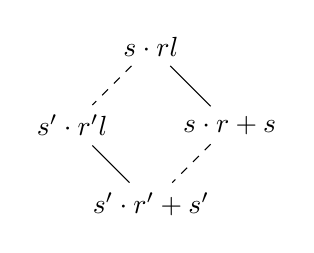
\begin{tikzpicture}
\node (A) at (0,0) {$s\cdot rl$};
\node (B) at (0,-2) {$s'\cdot r'+s'$};
\node (C) at (-1,-1) {$s'\cdot r'l$};
\node (D) at (1,-1) {$s\cdot r+s$};
\draw[dashed] (A) -- (C);
\draw (C) -- (B);
\draw (A) -- (D);
\draw[dashed] (D) -- (B);
\end{tikzpicture}}
\caption{Different forms of a diamond in computation paths}
\label{fig:loopdiamond}
\end{figure}

\begin{defi}[Simple variant computation paths, Homologous computation paths]
Two computation paths are \term[Simple variant computation paths]{simple variants} if they differ by a diamond, i. e. they look like figure \ref{fig:simplevariantshomologous}. Two paths are \term[Homologous computation paths]{homologous} if there is a sequence of computation paths $P_1,P_2,\ldots,P_n$ such that $P_1$ and $P_n$ are two paths in question and for $i=1,2,\ldots,n-1$, $P_i$ and $P_{i+1}$ are simple variants. Note that homologous paths assign the same value to a term.
\cite{conf/ijcai/Geiser75}
\end{defi}

\begin{figure}[hbt!]
\centering
\begin{tikzpicture}
\node (A) at (0,0) {$t$};
\node (B) at (0,-1) {$s$};
\node (C) at (0,-2) {$r$};
\node (D) at (0,-3) {$t'$};
\node (Dia) at (0,-1.5) {$\Diamond$};
\draw[dashed,->] (A) -- (B);
\draw[dashed] (B) edge[out=225,in=135,->] (C);
\draw[dashed] (B) edge[out=315,in=45,->] (C);
\draw[dashed,->] (C) -- (D);
\end{tikzpicture}
\caption{Simple variant computation paths}
\label{fig:simplevariantshomologous}
\end{figure}

\begin{defi}[Abstract ingredients of a term, Simple ingredients of a term, Raw material in an ingredient, Control element in an ingredient]
Let \sqnc{q_1}{q_2}{q_n} denote the occurrences of strokes in the term $t$. \funm{Ing}{t} denotes the set of list expressions obtained from \sqnc{q_1}{q_2}{q_n}, and $\cdot$,$\mbox{exp}$, according to the following rules.
\begin{enumerate}
 \item \sqnc{q_1}{q_2}{q_n} are in \funm{Ing}{t}
 \item If $\underline{i}$ and $\underline{j}$ are in \funm{Ing}{t} and $f$ is $\cdot$ or $\mbox{exp}$, then \tuple{\underline{i},\underline{j},f} is in \funm{Ing}{t}.
\end{enumerate}
The members of \funm{Ing}{t} are called the \term[Abstract ingredients of a term]{abstract ingredients} of $t$ and are called the \term[Simple ingredients of a term]{simple ingredients} of $t$. \fun{\mbox{Ing}_0}{t} is the set of simple ingredients of $t$. In \tuple{\underline{i},\underline{j},f}, $\underline{i}$ is the raw material and $\underline{j}$ is called the control element.
\cite{conf/ijcai/Geiser75}
\end{defi}

\begin{defi}[Homorphism]
A mapping \funsig{H}{\funm{Ing}{t}}{\funm{Ing}{t}} is a \termabbrev{homomorphism}{hom} \iffTx{} for all \tuple{\underline{i},\underline{j},f} in \funm{Ing}{t}:
\begin{equation}
\fun{H}{\tuple{\underline{i},\underline{j},f}} = \tuple{\fun{H}{\underline{i}},\fun{H}{\underline{j}},f}
\end{equation}
\cite{conf/ijcai/Geiser75}
\end{defi}

\begin{defi}[Real ingredient with respect to an evaluation path]
Let $P=\sqnc{t_1}{t_2}{t_n}$ be an evaluation path for $t$; thus $\abs{t}=t_n$. Define the homomorphism $\funf{H}{P}=\fun{H}{t_1\rightarrow t_2}\circ\fun{H}{t_2\rightarrow t_3}\circ\ldots\circ\fun{H}{t_{n-1}\rightarrow t_n}$ the set of \term[Real ingredient with respect to an evaluation path]{real ingredients with respect to $P$} is the set $\fun{\funf{H}{P}}{\fun{\mbox{Ing}_0}{t_n}}$ and is denoted \funm{Ing}{t;P}.
\cite{conf/ijcai/Geiser75}
\end{defi}

\begin{defi}[Equivalence relation for ingredients]
Let $\underline{i}$ and $\underline{j}$ be ingredients in \funm{Ing}{t}. We define \term[Equivalence relation for ingredients]{$\underline{i}\approx\underline{j}$} \iffTx{} there is a sequence of pairs \sqnc{\tuple{\underline{i}_1,\underline{j}_1}}{\tuple{\underline{i}_2,\underline{j}_2}}{\tuple{\underline{i}_n,\underline{j}_n}} of ingredients of \funm{Ing}{t} such that $\underline{i}=\underline{i}_n$, $\underline{j}=\underline{j}_n$ and for $k=\sqnc{1}{2}{n}$ either:
\begin{enumerate}
 \item $\underline{i}_k=\underline{j}_k$
 \item there exists ingredients $\underline{u}$, $\underline{v}$, $\underline{w}$ and function symbols $f$, $g$ such that \accol{\underline{i}_k,\underline{j}_k} equals \accol{\tuple{\tuple{\underline{u},\underline{v},f},\underline{w},g},\tuple{\tuple{\underline{u},\underline{w},g},\tuple{\underline{v},\underline{w},g},f}}, or
 \item there exists $k'$, $k''$ less than $k$ such that $\underline{i}_k=\tuple{\underline{i}_{k'},\underline{i}_{k''},f}$ and $\underline{j}_k=\tuple{\underline{j}_{k'},\underline{j}_{k''},f}$.
\end{enumerate}
\cite{conf/ijcai/Geiser75}
\end{defi}

\begin{defi}[Skeptical explanation of a literal, Minimal explanation of a literal]
Let $P$ be a consistent Extended Logic Program, and $O$ a literal. Suppose that $\Psi$ is a set of candidate priorities on $\calL_p$. A set $\psi$ of priorities is a \term[Skeptical explanation of a literal]{(skeptical) explanation of $O$} (\wrtTx{} \accol{P,\Psi}) if
\begin{enumerate}
 \item $\psi\subseteq\Psi$, and
 \item $P\vDash_\psi O$.
\end{enumerate}
Also, $\psi$ is a \term[Minimal explanation of a literal]{minimal explanation of $O$} if no $\psi'\subset\psi$ is an explanation of $O$.
\cite{conf/ijcai/InoueS99}
\end{defi}

\begin{defi}[Preference abduction framework, Skeptical explanation of a literal, Minimal explanation of a literal]
A \term{preference abduction framework} is a triple \tuple{P,\Gamma,\Psi} where P is an Extended Logic Program, $\Gamma\subseteq\calL_P$ is a set of abducibles, and $\Psi$ is a set of candidate priorities on $\calL_P$. A pair \tuple{A,\psi} is a \term[Skeptical explanation of a literal]{(skeptical) explanation of a literal $O$} (\wrtTx{} \tuple{P,\Gamma,\Psi}) if
\begin{enumerate}
 \item $A\subseteq\Gamma$,
 \item $\psi\subseteq\Psi$,
 \item $P\cup A$ is consistent, and 
 \item $P\cup A\vDash_\psi O$
\end{enumerate}
Also \tuple{A,\psi} is a \term[Minimal explanation of a literal]{minimal explanation of $O$} if for any explanation \tuple{A',\psi'} of $O$, $A'\subseteq A$ and $\psi'\subseteq\psi$ imply $A'=A$ and $\psi'=\psi$.
\cite{conf/ijcai/InoueS99}
\end{defi}

\subsection{Proof Normalization}

\begin{defi}[Discharged assumptions by the rule]
At applications of $\supset I$, $\exists E$ and $\mbox{IND}$ rules, certain assumptions are said to be ``\term[Discharged assumptions by the rule]{discharged}'' by the rule. The conclusion of a proof is said to depend on the assumptions that have not been discharged.
\cite{conf/ijcai/Goto85}
\end{defi}

\begin{defi}[Proper parameter of the inference rule]
In applications of the rule $\forall I$, $\exists E$ and $\mbox{IND}$, the variable ``a'' (see figure \ref{fig:properparameteroftheinferencerule}) is called the \term{proper parameter of the inference rule}.
\cite{conf/ijcai/Goto85}
\end{defi}

\begin{figure}[hbt]
\centering
\begin{tikzpicture}
\begin{scope}[xshift=0cm,yshift=0cm]
\node[anchor=south] (A) at (-0.5,0) {$A$};
\node[anchor=south] (B) at (0.5,0) {$B$};
\node[anchor=west] (O) at (B.south east) {$\wedge I$};
\node[anchor=north] (R) at (0,0) {$A\wedge B$};
\draw (A.south west) -- (B.south east);
\end{scope}
\begin{scope}[xshift=4cm,yshift=0cm]
\node[anchor=south] (B) at (0,0) {$A\wedge B$};
\node[anchor=west] (O) at (B.south east) {$\wedge E$};
\node[anchor=north] (R) at (0,0) {$A$};
\draw (B.south west) -- (B.south east);
\end{scope}
\begin{scope}[xshift=8cm,yshift=0cm]
\node[anchor=south] (B) at (0,0) {$B$};
\node[anchor=south] (Bsup) at (B.north) {$\flatbrak{A}$};
\draw (Bsup.south west) -- (Bsup.south east);
\node[anchor=north] (R) at (0,0) {$A\supset B$};
\draw (R.north west) -- (R.north east);
\node[anchor=west] (O) at (R.north east) {$\supset I$};
\end{scope}
\begin{scope}[xshift=12cm,yshift=0cm]
\node[anchor=south] (A) at (-0.5,0) {$A$};
\node[anchor=south] (B) at (0.5,0) {$A\supset B$};
\node[anchor=west] (O) at (B.south east) {$\supset E$};
\node[anchor=north] (R) at (0,0) {$B$};
\draw (A.south west) -- (B.south east);
\end{scope}
\begin{scope}[xshift=0cm,yshift=-2cm]
\node[anchor=south] (B) at (0,0) {$\fun{A}{a}$};
\node[anchor=north] (R) at (0,0) {$\fun{\forall x}{\fun{A}{x}}$};
\draw (R.north west) -- (R.north east);
\node[anchor=west] (O) at (R.north east) {$\forall I$};
\end{scope}
\begin{scope}[xshift=4cm,yshift=-2cm]
\node[anchor=south] (B) at (0,0) {$\fun{\forall x}{\fun{A}{x}}$};
\node[anchor=west] (O) at (B.south east) {$\forall E$};
\node[anchor=north] (R) at (0,0) {$\fun{A}{a}$};
\draw (B.south west) -- (B.south east);
\end{scope}
\begin{scope}[xshift=8cm,yshift=-2cm]
\node[anchor=south] (B) at (0,0) {$\fun{A}{t}$};
\node[anchor=north] (R) at (0,0) {$\fun{\exists x}{\fun{A}{x}}$};
\draw (R.north west) -- (R.north east);
\node[anchor=west] (O) at (R.north east) {$\exists I$};
\end{scope}
\begin{scope}[xshift=12cm,yshift=-2cm]
\node[anchor=south] (A) at (-0.75,0) {$\fun{\exists x}{\fun{A}{x}}$};
\node[anchor=south] (B) at (0.75,0) {$C$};
\node[anchor=south] (Bsup) at (B.north) {$\flatbrak{\fun{A}{a}}$};
\draw (Bsup.south west) -- (Bsup.south east);
\node[anchor=west] (O) at (B.south east -| Bsup.south east) {$\exists E$};
\node[anchor=north] (R) at (0,0) {$C$};
\draw (A.south west) -- (B.south east -| Bsup.south east);
\end{scope}
\begin{scope}[xshift=6cm,yshift=-4cm]
\node[anchor=south] (A) at (-0.75,0) {$\fun{A}{0}$};
\node[anchor=south] (B) at (0.75,0) {$\fun{A}{\fun{s}{a}}$};
\node[anchor=south] (Bsup) at (B.north) {$\flatbrak{\fun{A}{a}}$};
\draw (Bsup.south west) -- (Bsup.south east);
\node[anchor=west] (O) at (B.south east -| Bsup.south east) {$\mbox{IND}$};
\node[anchor=north] (R) at (0,0) {$\fun{A}{t}$};
\draw (A.south west) -- (B.south east -| Bsup.south east);
\end{scope}
\end{tikzpicture}
\caption{Inference rules in natural deduction.}
\label{fig:properparameteroftheinferencerule}
\end{figure}

\begin{defi}[Normal proof]
A proof $\Pi$ is said to be \term[Normal proof]{normal}, if no reduction rule is applicable to $\Pi$.
\cite{conf/ijcai/Goto85}
\end{defi}

\begin{defi}[Harrop formula class]
The \term[Harrop formula class]{class of Harrop formulas} is defined inductively as follows:
\begin{enumerate}
 \item Every atomic formula is a Harrop formula
 \item If $A$ and $B$ are Harrop formula's, then $A\wedge B$ and $\fun{\forall x}{\fun{A}{x}}$ are Harrop formulas.
 \item If $B$ is a Harrop formula, then $A\supset B$ is a Harrop formula, regardless of the form of $A$.
\end{enumerate}
\cite{conf/ijcai/Goto85}
\end{defi}

\section{Critical Reasoning}

\begin{defi}[Critical Environment]
The \term{critical environment} for node $n$ relative to $S\subseteq A$ is:
\begin{equation}
\fun{\hat{S}}{n}=\displaystyle\bigcap\accol{E\in\fun{\calE}{n}|E\subseteq S}
\end{equation}
\cite{conf/ijcai/RaimanKS93}
\end{defi}

\begin{defi}[Critical Conflict]
The \term{critical conflict} for $S\subseteq\calA$ is:
\begin{equation}
\fun{\hat{S}}{\bot}=\displaystyle\bigcap\accol{C\mbox{ a conflict}|C\subseteq S}
\end{equation}
\cite{conf/ijcai/RaimanKS93}
\end{defi}

\begin{defi}[Critical abstraction of a theory]
The \term{critical abstraction of a theory} $\calT$ relative to $S\subseteq A$ is the theory:
\begin{equation}
\fun{\hat{S}}{\calT}=\calT\cup\accol{\fun{\hat{S}}{n}\rightarrow n|n\in\calL\cup\accol{\bot}}
\end{equation}
\cite{conf/ijcai/RaimanKS93}
\end{defi}

\begin{defi}[Critical cover]
A \term{critical cover} relative to a subset $S$ of $\calA$ is a set $\accol{S_1,S_2,\ldots,S_k}$ of subsets of $S$ such that:
\begin{enumerate}
 \item \term[Critical consistency in critical cover]{Critical consistency}: $\fun{\hat{S}_i}{\bot}$ is non-empty, for all $i$.
 \item \term[Covering in critical cover]{Covering}: Every conflict $C\subseteq S$ is subsumed by $\fun{\hat{S}_i}{\bot}$, for some $i$.
 \item \term[Disjointness in critical cover]{Disjointness} $\fun{\hat{S}_i}{\bot}$ is disjoint from $S_j$, far every distinct $i$ and $j$.
\end{enumerate}
\cite{conf/ijcai/RaimanKS93}
\end{defi}

\begin{defi}[Critical diagnosis] A \term{critical diagnosis} of $\calT$ relative to a $S\subseteq\calA$ is a set $\Delta\cap\bar{S}$ such that:
\begin{enumerate}
 \item $\Delta$ is a diagnosis of \fun{\hat{S}}{\calT}.
 \item There is no other diagnosis $\Delta'$ of \fun{\hat{S}}{\calT}, such that $\Delta'\cap\bar{S}$ is a strict subset of $S\subseteq\calA$.
\end{enumerate}
\cite{conf/ijcai/RaimanKS93}
\end{defi}

\section{Argumentation}

\begin{defi}[Argumentation framework, Arguments in an argumentation framework]
An \term{argumentation framework} is a pair $AF=\tuple{\calA,\calR}$ where $\calA$ is a set of \term[Arguments in an argumentation framework]{arguments}, and $\calR$ is a binary relation representing a defeat relationship between arguments, i.e. $\calR\subseteq\calA\times\calA$. $\brak{A,B}\in\calR$ or equivalently "$A\calR B$" means that argument $A$ defeats argument $B$. We also say "$A$ attacks $B$". Here an argument is an abstract entity whose role is only determined by its relation to other arguments.
\cite{conf/ijcai/Dung93}
\end{defi}

\begin{defi}[Acceptable argument with respect to a set of arguments,Admissible conflict-free set of arguments]
\begin{enumerate}
 \item An argument $A$ is \term[Acceptable argument with respect to a set of arguments]{acceptable \wrtTx{} a set $S$ of arguments} \iffTx{} for each argument $B$: if $B$ attacks $A$ then $B$ is attacked by some argument in $S$.
 \item A conflict-free set of arguments $S$ is \term[Admissible conflict-free set of arguments]{admissible} \iffTx{} each argument in $S$ is acceptable \wrtTx{} $S$.
\end{enumerate}
\cite{conf/ijcai/Dung93}
\end{defi}

\begin{defi}[Maximal preferred extension of an argumentation framework]
A \term{preferred extension of an argumentation framework} $AF$ is a maximal (\wrtTx{} set inclusion) admissible set of arguments of $AF$.
\cite{conf/ijcai/Dung93}
\end{defi}

\begin{defi}[Stable extension]
A conflict-free set of arguments $S$ is called a \term{stable extension} \iffTx{} $S$ attacks each argument which does not belong to $S$.
\cite{conf/ijcai/Dung93}
\end{defi}

\begin{defi}[Characteristic function of an argumentation framework]
The \term{characteristic function of an argumentation framework} $AF=\tuple{\calA,\calR}$ denoted by $F_{AF}$, is defined as follows: \funsig{F_{AF}}{2^{\calA}}{2^{\calA}} where $\fun{F_{AF}}{S}=\accol{A|A\mbox{ is acceptable \wrtTx{} }S}$.
\cite{conf/ijcai/Dung93}
\end{defi}

\begin{defi}[Grounded extension of an argumentation framework]
The \term{grounded extension of an argumentation framework} $AF$, denoted by $G_{AF}$, is the least fixed point of $F_{AF}$.
\cite{conf/ijcai/Dung93}
\end{defi}

\begin{defi}[Complete extension]
An admissible set of arguments $S$ is called a \term{complete extension} \iffTx{} each argument which is acceptable \wrtTx{} $S$, belongs to $S$.
\cite{conf/ijcai/Dung93}
\end{defi}

\section{Explanation Based Learning}

\begin{defi}[Explanation structure, Internal structure of an explanation structure, External structure of an explanation structure, Instantiation of an explanation structure, Uninstanstiation of an explanation structure, Binary resolvent of two explanation structures, Unresolution of an explanation structure, Remainder of an explanation structure, Generalization of an explanation structure]
\begin{enumerate}
 \item For a horn clause $C=A\leftarrow B_1\wedge B_2\wedge\ldots\wedge B_n$ let it's equivalent copy be $C'=A'\leftarrow B_1'\wedge B_2'\wedge\ldots\wedge B_n'$. Then the following expression is an \term{explanation structure}.
 \begin{equation}
  A':\brak{A\leftarrow \brak{B_1:B_1'}\wedge\brak{B_2:B_2'}\wedge\ldots\wedge\brak{B_n:B_n'}}
 \end{equation}
 $C$ and $C'$ are called its \term[Internal structure of an explanation structure]{internal} and \term[External structure of an explanation structure]{external structure} respectively.
 \item For an explanation structure $T$, let $C'$ be its external structure and $\sigma$ be a substitution. Then, the expression $T\sigma$, which has the same internal structure as $T$ and has
the external structure $C'\sigma$ is called an \term[Instantiation of an explanation structure]{instantiation of $T$}. Inversely, $T$ is called an \term[Uninstanstiation of an explanation structure]{uninstantiation of $T\sigma$}.
 \item For two explanation structures $S$ and $T$, let $A'\leftarrow B_1'\wedge B_2'\wedge\ldots\wedge B_n'$ and $B_i'\leftarrow C_1'\wedge C_2'\wedge\ldots\wedge C_m'$ be their external structures respectively. Then, the expression $U$ connected $S$ and $T$ at $B_i'$ is called a \term[Binary resolvent of two explanation structures]{(binary) resolvent of $S$ and $T$}. Inversely $S$ is called the \term[Unresolution of an explanation structure]{unresolution of $U$} and $T$ is called the \term[Remainder of an explanation structure]{remainder}.
 \item An explanation structure $S$ is \term[Generalization of an explanation structure]{more general} than $T$ denoted by $S\preceq T$ \iffTx{} there exists a sequence of uninstantiations and unresolutions from $T$ to $S$.
\end{enumerate}
\cite{conf/ijcai/YamamuraK91}
\end{defi}

\begin{defi}[Obliged generalization of an explanation structure, EBG, EBG Macro]
\begin{enumerate}
 \item An explanation $T$ is an \term{obliged generalization}, \iffTx{} the internal structure of T does not include any facts of a certain example and its external structure is a definite clause.
 \item Obliged generalizations of an explanation for some example are called \term{EBG}. For an EBG, its external structure is called an \term{EBG macro}.
\end{enumerate}
\cite{conf/ijcai/YamamuraK91}
\end{defi}

\begin{defi}[More general explanation, Generalization space]
\begin{enumerate}
 \item For an explanation $T\in\calT$, let $T_0$ be an uninstantiation of $T$. Then $\calT'=\brak{\calT\setminus\accol{T}}\cup\accol{T_0}$ is an uninstantiation of $T$. Similarly let $T_0$ be an unresolution and $T_0,T_1,\ldots,T_n$ are its remainders. Then $\calT'=\brak{\calT\setminus\accol{T}}\cup\accol{T_1,T_2,\ldots,T_n}$ is an unresolution of $\calT$.
 \item An explanation $S$ is \term[More general explanation]{more general} than $T$, denoted by $S<T$ \iffTx{} there exists a sequence of uninstantiations and unresolutions from $T$ to $S$.
 \item A class of all generalizations of the obliged general of an example set is called a \term{generalization space}.
\end{enumerate}
\cite{conf/ijcai/YamamuraK91}
\end{defi}

\begin{defi}[Common EGB, Least EBG]
For EBGs $T_1,\ldots,T_n$, $T$ is a \term{common EBG} \iffTx{} $T\preceq T_1,T\preceq T_2,\ldots,T\preceq T_n$. The least generalization in common EBGs is called the \term{least EBG}.
\cite{conf/ijcai/YamamuraK91}
\end{defi}

\begin{defi}[Least EGB generalization of an explanation, More general by least EBG, Least EBG space]
\begin{enumerate}
 \item For $\calS\subseteq\calT$, let $T_0$ be the least EBG of $\calS$ and $T_1,T_2,\ldots,T_n$ be its remainder. Then $\calT'=\brak{\calT\subseteq S}\cup\accol{T_0,T_1,\ldots,T_n}$ is called a \term[Least EGB generalization of an explanation]{least EBG generalization} of $\calT$.
 \item $\calS$ is \term{more general by least EBG than} $\calT$ \iffTx{} there exists a sequence of least EBG generalizations from $\calT$ to $\calS$.
 \item A class of all least EBG generalizations of the obliged generalization of an example set is called its \term{least EBG space}.
\end{enumerate}
\cite{conf/ijcai/YamamuraK91}
\end{defi}

\begin{defi}[Usage degree, Backtrack number \fun{\calB}{\calT,\calE}, Operationally criteria for generalizations]
\begin{enumerate}
 \item For a generalization $\calS=\brak{\calT\setminus\accol{T}}\cup\accol{T_0,T_1,\ldots,T_n}$, its \term{usage degree} is a function \stTx{}
 \begin{equation}
  \fun{\calU}{\calS,\calT}=\displaystyle\sum_{i=0}^{n}{\left\{\begin{array}{ll}
  \abs{T_i}&\mbox{if }T_i\in\calT\\0&\mbox{otherwise}\end{array}\right.}
 \end{equation}
 Where $\abs{T_i}$ denotes the number of clauses used in $T_i$. In general, when $\calS\preceq\calT$, the usage degree sums up all usage degrees through some generalization path.
 \item For an example set $\calE$ and its generalization $\calT$, the \term{backtrack number \fun{\calB}{\calT,\calE}} is the minimum of the sum of goal failures which occur during a macrotable of $\calT$ reconstructs all explanations of $\calE$.
 \item  For two generalizations $\calS$ and $\calT$ of an example set $\calE$, $\calS$ is \term[Operationally criteria for generalizations]{more operational than} $\calT$ \iffTx{} and $\fun{\calU}{\calS,\calE}\geq\fun{\calU}{\calT.\calE}$ and $\fun{\calB}{\calS,\calE}\geq\fun{\calB}{\calT.\calE}$.
\end{enumerate}
\cite{conf/ijcai/YamamuraK91}
\end{defi}

\section{Transformation Problems}

\subsection{Termination}

\begin{defi}[type-1-separated subset]
$S_1$ is a \term{type-1-separated subset} of $S$ \iffTx{} \faTx{} $f\in F$ and all $s\in S_1\cap S_f$, $\ffun{s}\in S_1$.
\cite{conf/ijcai/Florath75}
\end{defi}

\begin{defi}[type-2-separated subset]
$S_1$ is a \term{type-2-separated subset} of $S$ \iffTx{} \faTx{} $f\in F$ and all $s\in \brak{S\setminus S_1}\cap S_f$, $\ffun{s}\in S\setminus S_1$.
\cite{conf/ijcai/Florath75}
\end{defi}

\begin{defi}[type-3-separated subset]
$S_1$ is a \term{type-3-separated subset} of $S$ \iffTx{} $S_1$ is both a type-1-separated subset and type-2-separated subset of $S$.
\cite{conf/ijcai/Florath75}
\end{defi}

\begin{defi}[Consistent type-$k$-system of subsets]
$\gamma$ is a \term{consistent type-$k$-system of subsets} of $S$ \iffTx{} \faTx{} $s_1\in S$, $s_2\in S$ the statement defined by decision rule $k$ is true.
\cite{conf/ijcai/Florath75}
\end{defi}

\begin{defi}[admissible type-$k$-system of subsets]
$\gamma$ is an \term{admissible type-$k$-system of subsets} of $S$ \iffTx{} \faTx{} $s1,s_2\in S$, the following is true: $\brak{s_1,s_2}$ is solvable \iffTx{} \faTx{} $S_i\in\gamma$ holds condition $C_k$ where $C_1$, $C_2$ and $C_3$ are defined as follows:
\begin{description}
 \item [$C_1$] $s_1\in S_i$ implies $s_2\in S_i$.
 \item [$C_2$] $s_2\in S_i$ implies $s_1\in S_i$.
 \item [$C_3$] $s_1\in S_i$ \iffTx{} $s_2\in S_i$.
\end{description}
\cite{conf/ijcai/Florath75}
\end{defi}

\begin{defi}[Cycle within an operator set of a conjunctive problem space]
Within the operator set $F$ of a conjunctive problem space, there is a \term[Cycle within an operator set of a conjunctive problem space]{cycle} with respect to the relation $\succ$ \iffTx{} there are operators $f_{i_1},f_{i_2},\ldots,f_{i_l}$ such that $f_{i_1}\succ f_{i_2}\succ\ldots\succ f_{i_l}$.
\cite{conf/ijcai/Florath75}
\end{defi}

\section{Epistemic State}

\begin{defi}[Epistemic state, Admissible belief states]
An \term{epistemic state} $\pounds$ is a triple $\tuple{S,\prec,l}$, where $S$ is a set of objects called \term{admissible belief states}, $\prec$ is a preference relation on $S$, while $l$ is a labeling function assigning each admissible state a deductively closed theory.
\cite{conf/ijcai/Bochman99}
\end{defi}

\begin{defi}[Sceptically valid in an epistemic state]
A conditional $A\dashsim B$ will be said to be \term{sceptically valid in an epistemic state} $\pounds$ if all preferred states in $\brak{A}$ support $A\rightarrow B$.
\cite{conf/ijcai/Bochman99}
\end{defi}

\begin{defi}[Credulously valid in an epistemic state]
A conditional $A\dashsim B$ will be said to be \term{credulously valid in an epistemic state} $\pounds$ if either $\brak{A}$ is empty or at least one preferred state in $\brak{A}$ supports $A\rightarrow B$.
\cite{conf/ijcai/Bochman99}
\end{defi}

\begin{defi}[Credulous nonmonotonic inference relation, Rational monotony]
A nonmonotonic inference relation will be called \term[Credulous nonmonotonic inference relation]{credulous} if it is regular and satisfies \term{Rational Monotony}:
\begin{equation}
\brak{\mbox{RM}}\mbox{ If }A\dashsim B\mbox{ and } A\negdashsim C\mbox{, then } A\wedge C\dashsim B
\end{equation}
\cite{conf/ijcai/Bochman99}
\end{defi}

\begin{defi}[Permissive inference relation, Cut rule, Or rule]
An inference relation will be called \term[Permissive inference relation]{permissive} if it satisfies the basic postulates and the \term{Cut rule}:
\begin{equation}
\brak{\mbox{Cut}}\mbox{ If }A\dashsim B\mbox{ and } A\wedge B\dashsim C\mbox{, then } A\dashsim C
\end{equation}
It can be shown that, in the context of $B$, Cut implies the \term[Or rule]{rule Or}:
\begin{equation}
\brak{\mbox{Or}}\mbox{ If }A\dashsim C\mbox{ and } B\dashsim C\mbox{, then } A\vee B\dashsim C
\end{equation}
\cite{conf/ijcai/Bochman99}
\end{defi}

\begin{defi}[Permissively valid conditional in an epistemic state]
A conditional $A\dashsim B$ will be said to be \term[permissively valid conditional in an epistemic state]{permissively valid in an epistemic state} $\pounds$ if any preferred state in $\brak{A}$ is consistent with $A\wedge B$.
\cite{conf/ijcai/Bochman99}
\end{defi}

\section{Temporal Reasoning}

\begin{defi}[Specification of a document]
A \term[Specification of a document]{specification} $s=\tuple{O,C}$ of a document is made of a set of objects $O$ and a set of constraints $C$ between these objects (i.e., a relation between several objects). The set of all specifications will be noted $S$.
\cite{conf/ijcai/EuzenatLD03}
\end{defi}

\begin{defi}[Relation graph of a specification]
A specification $s=\tuple{O,C}$ can be represented as a complete direct labeled graph called a \term[Relation graph of a specification]{relation graph} $g_s=\tuple{N,E,\lambda}$ such that the elements of $O$ are in bijection with those of $N$ and \funsig{\lambda}{E}{2^{A_{13}}} is a total function from the arcs to temporal relations such that for each $x\ r\ y\in C$, $\fun{\lambda}{\tuple{x,y}}\subseteq r$.
\cite{conf/ijcai/EuzenatLD03}
\end{defi}


\begin{defi}[Resolved relation graph of a specification].
A relation graph is \term[Resolved relation graph of a specification]{resolved} \iffTx{} all the labels are singletons.
\cite{conf/ijcai/EuzenatLD03}
\end{defi}

\begin{defi}[Interpretation of a specification]
An \term{interpretation of a specification} is a pair \tuple{I,D} such that $D$ is the domain of interpretation and $I$ is a function from $O$ to $D$ and from $C$ to $D\times D$ (i.e., such that a constraint applied to two elements of the domain of interpretation is either true of false).
\cite{conf/ijcai/EuzenatLD03}
\end{defi}

\begin{defi}[Temporal interpretation of a specification]
in order to \term[Temporal interpretation of a specification]{interpret the temporal aspects} of multimedia documents, we consider the interpretations such that the objects in $O$ are interpreted as intervals of the positive real numbers and the constraints are interpreted as the corresponding relations in the temporal interval algebra.
\cite{conf/ijcai/EuzenatLD03}
\end{defi}

\begin{defi}[Model of a specification]
A model of a specification \tuple{O,C} is an interpretation \tuple{I,D} such that for each $o\ r\ o'\in C$. $\tuple{\fun{I}{o},\fun{I}{o'}}\in\fun{I}{r}$ is true. The set of models of a specification $s$ is noted $\calM_s$.
\cite{conf/ijcai/EuzenatLD03}
\end{defi}

\begin{defi}[Qualitative representation of a model of a specification].
The \term[Qualitative representation of a model of a specification]{qualitative representation of a model} \tuple{I,D} of a specification \tuple{O,C} is a complete direct labeled graph \tuple{N,E,\lambda} such that the elements of $O$ are in bijection with those of $N$ and \funsig{\lambda}{E}{2^{A_{13}}} is a total function from the arcs to temporal relations such that for each $\fun{I}{x}\ r\ \fun{I}{y}$, $\fun{\lambda}{\tuple{x,y}}=r$.
\cite{conf/ijcai/EuzenatLD03}
\end{defi}

\begin{defi}[Adaptation constraint].
An \term{adaptation constraint} $a$ determines a set of possible executions $M_a$. The set of adaptation constraints will be noted $A$.
\cite{conf/ijcai/EuzenatLD03}
\end{defi}

\begin{defi}[Classification of adaptation, Compliant specification, Refining adaption, Transgressive adaption]
Three types of adaptation can be identified in function of the value of $\calM_s\cap\calM_p$ (inducing three different constraints on the model selection function $\alpha$):
\begin{description}
 \item [\term{Compliant specification}] $\calM_s\cap\calM_p=\calM_s$,: the source document satisfies the adaptation constraints (all models of $\calM_s$, satisfy the adaptation constraints. so $\alpha$ is identity).
 \item [\term{Refining adaptation}] $\emptyset\subset\calM_s\cap\calM_p\subset\calM_s$: there exists some models of $s$ satisfying the adaptation constraints ($\fun{\alpha}{\calM_s}=\calM_s\cap\calM_p$).
 \item [\term{Transgressive adaptation}] $\calM_s\cap\calM_p=\emptyset$: no model of $s$ satisfies the adaptation constraints ($\alpha$ will then select some models of $\calM_p$, closest to those of the specification $s$).
\end{description}
\cite{conf/ijcai/EuzenatLD03}
\end{defi}

\begin{defi}[Distance between sets of models]
The \term{distance between sets of models} is defined as:
\begin{equation}
\fun{\Delta}{\calM,\calM'}=F_{m\in\calM,m'\in\calM'}\fun{d}{m,m'}
\end{equation}
\cite{conf/ijcai/EuzenatLD03}
\end{defi}

\begin{defi}[Distance between resolved relation graphs]
The \term{distance between resolved relation graphs} is defined as:
\begin{equation}
\fun{d}{\lambda,\lambda'}=\displaystyle\sum_{n,n'\in N}\left\{\begin{array}{ll}
1&\mbox{if }\fun{\lambda}{\tuple{n,n'}}\neq\fun{\lambda'}{\tuple{n,n'}}\\
0&\mbox{otherwise}
\end{array}\right.
\end{equation}
\cite{conf/ijcai/EuzenatLD03}
\end{defi}

\begin{defi}[Distance between interval relations based on endpoints]
The \term{distance between interval relations based on endpoints} is defined as:
\begin{equation}
\fun{\delta}{r,r'}=\displaystyle\sum_{i=1}^4\left\{\begin{array}{ll}
1&\mbox{if }\fun{\gamma}{r}\flatbrak{i}\neq\fun{\gamma}{r'}\flatbrak{i}\\
0&\mbox{otherwise}
\end{array}\right.
\end{equation}
\cite{conf/ijcai/EuzenatLD03}
\end{defi}

\begin{defi}[Distance between models based on endpoints]
The \term{distance between models based on endpoints} is defined as:
\begin{equation}
\fun{d}{\lambda,\lambda'}=\displaystyle\sum_{n,n'\in N}\fun{\delta}{\fun{\lambda}{\tuple{n,n'}},\fun{\lambda'}{\tuple{n,n'}}}
\end{equation}
\cite{conf/ijcai/EuzenatLD03}
\end{defi}

\begin{defi}[Conceptual neighborhood relation]
The \term{conceptual neighborhood relation} is a binary relation $N_{\Gamma}^X$ between elements of a set of relations $\Gamma$ such that $\fun{N_{\Gamma}^X}{r,r'}$ \iffTx{} the continuous transformation $X$ of a situation involving two individuals $x$ and $y$ can transform $\fun{r}{x,y}$ into $\fun{r'}{x,y}$ without transiting by a third relation.
\cite{conf/ijcai/EuzenatLD03}
\end{defi}

\begin{defi}[Conceptual distance between two relations]
The \term[Conceptual distance between two relations]{conceptual distance $\delta'$ between two relations} is the length of the shortest path between $r$ and $r'$ in the graph of $N_{\Gamma}^X$.
\cite{conf/ijcai/EuzenatLD03}
\end{defi}

\begin{defi}[Conceptual distance between models]
The \term{conceptual distance between models} is defined as:
\begin{equation}
\fun{d}{\lambda,\lambda'}=\displaystyle\sum_{n,n'\in N}\fun{\delta'}{\fun{\lambda}{\tuple{n,n'}},\fun{\lambda'}{\tuple{n,n'}}}
\end{equation}
\cite{conf/ijcai/EuzenatLD03}
\end{defi}

\section{Model Ranking}

\begin{defi}[Robust with respect to a set of defaults]
An integer ranking $\kappa$, over models is said to be \term{robust with respect to a set of defaults} \accol{r_i}, with associated strengths \accol{s_i}, if no two defaults share a common minimal falsifying model in $\kappa$.
\cite{conf/ijcai/BourneP99}
\end{defi}

\begin{defi}[Me-valid integer ranking]
An integer ranking $\kappa$, over $\alpha$ set of defaults \accol{r_i}, with associated strengths \accol{s_i}, is said to be \term[Me-valid integer ranking]{me-valid} with respect to that set if it satisfies
\begin{equation}
\fun{\kappa}{m}=\displaystyle\sum_{\frac{r_i}{m\vDash a_i\wedge\neg b_i}}{\fun{\kappa}{r_i}}
\end{equation}
and for all $r$
\begin{equation}
\fun{\kappa}{v_r}+s_r=\fun{\kappa}{f_r}
\end{equation}
\cite{conf/ijcai/BourneP99}
\end{defi}

1\begin{defi}[Distinct me-valid integer rankings]
Two me-valid rankings, $\kappa$ and $\kappa'$ are said to be \term[Distinct me-valid integer rankings]{distinct} \iffTx{} $\fun{\kappa}{r}\neq\fun{\kappa'}{r}$ for some default $r$. Such a default is said to be distinctly ranked.
\cite{conf/ijcai/BourneP99}
\end{defi}